%!TEX program = xelatex
% 完整编译: xelatex -> biber/bibtex -> xelatex -> xelatex
\documentclass[lang=cn,11pt,a4paper]{elegantpaper}

\title{viscosity.h文档说明}
\author{Haochen Huang}
\institute{西安交通大学MFM课题组}

\version{2.02test}
\date{\zhtoday}


% 本文档命令
\usepackage{array}

\begin{document}

\maketitle
\tableofcontents

\begin{abstract}
本文为basilisk的头文件viscosity.h的说明文档,请注意,在阅读此文当前应当完整阅读poisson.h说明文档。\par
2.02更新,纠正公式细节问题,调整文章顺序,新添加程序参数调用图例。
\end{abstract}


\section{理论背景}

\subsection{文件目的}
该文档目的为利用poisson.h头文件中建立的迭代方法求解扩散方程
\begin{equation}\label{equ:main}
    \rho_{n+\frac{1}{2}}[\frac{\mathbf{u^*-u^{***}}}{\Delta t}]=\nabla\cdot[2\mu_{n+\frac{1}{2}}\mathbf{D^*}]
\end{equation}
上式中需要求解的未知量为$u^*$,其余量如$u^{***}$已知,方程右端进行插值可以得到相应表达式。\par
poisson.h中已经构建了相应的求解算法,我们需要做的是重新构建表达未知量与已知量之间关系的relax函数,以及计算相应残差的residual函数,从而组成求解扩散方程的求解器。\par
其基本的代码框架如下,图中表达的主要是各类主要参数的来回传递,便于读者对照,每个主体参数联系之间使用了不同颜色。
\begin{figure}[H]
    \centering
    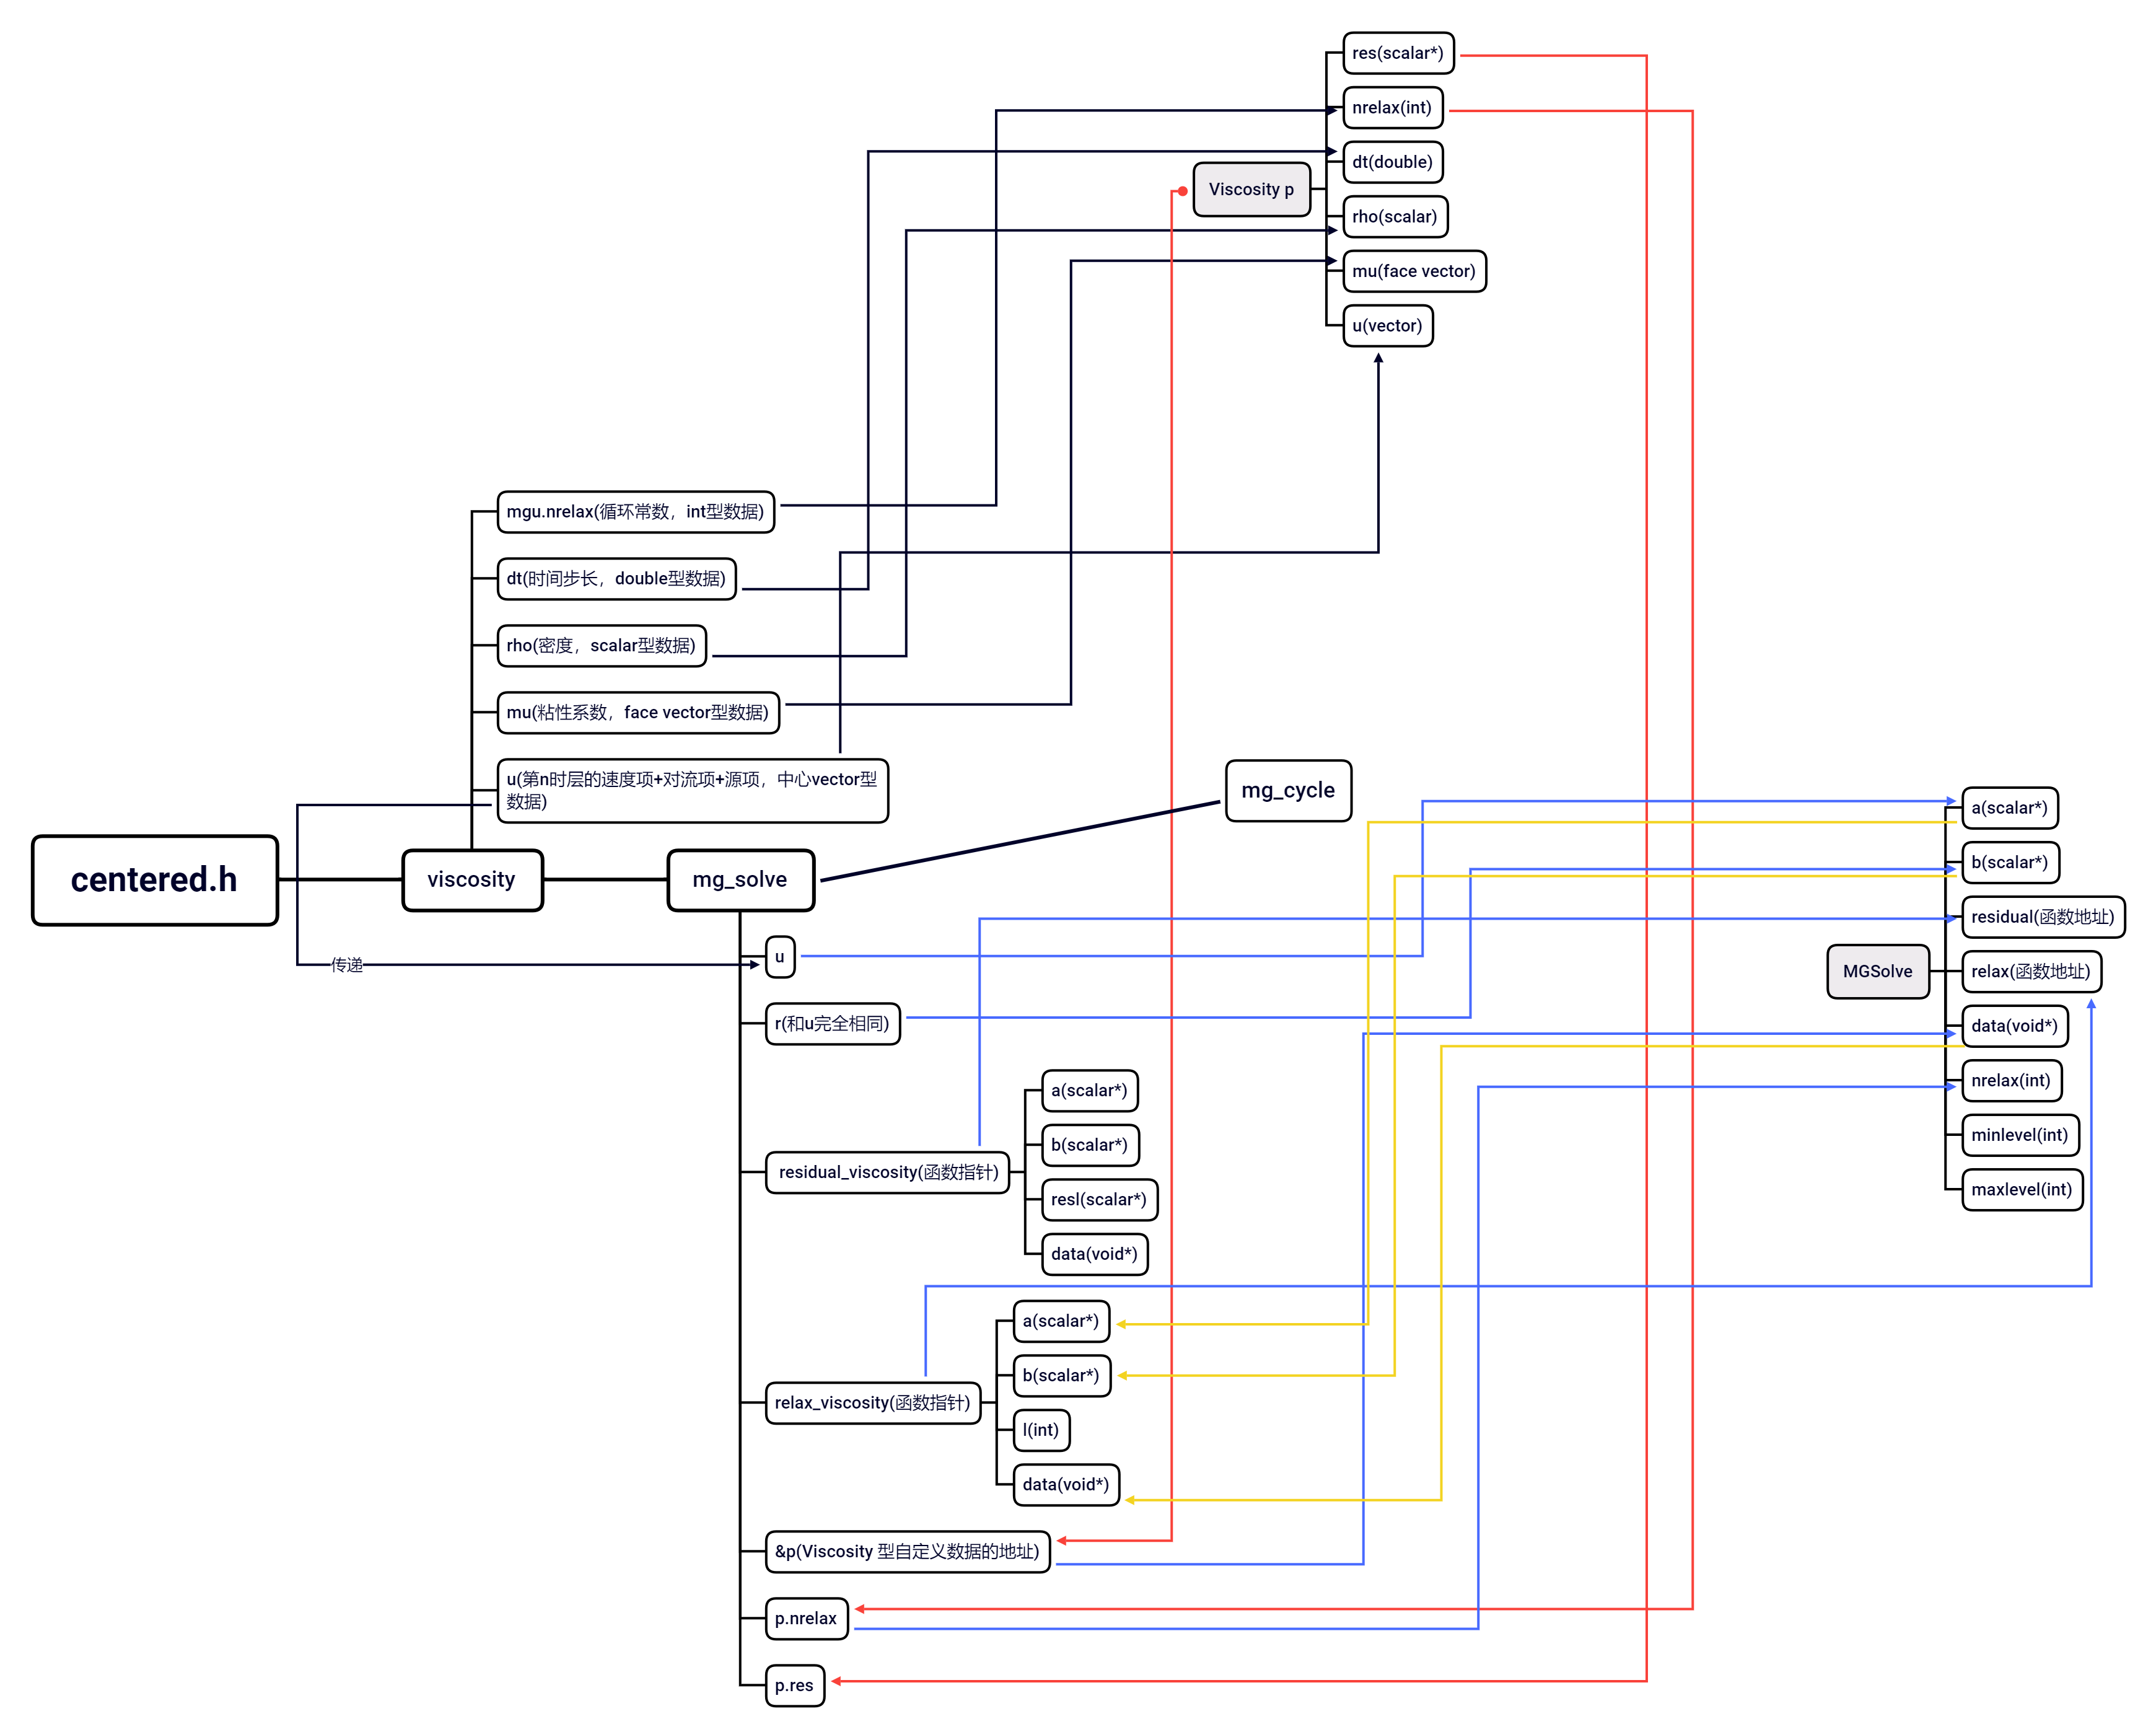
\includegraphics[width=1.0\linewidth]{viscosity.png}
    \caption{程序参数调用图例}
    \label{fig:kuangjia}
\end{figure}
\subsection{扩散项离散格式}
对\ref{equ:main}两端在单元内进行积分有
\begin{equation}
    \int_{C}\rho_{n+\frac{1}{2}}[\frac{\mathbf{u^*-u^{***}}}{\Delta t}]dV=\int_{C}\nabla\cdot[2\mu_{n+\frac{1}{2}}\mathbf{D^*}] dV= \int_{\partial C}[2\mu_{n+\frac{1}{2}}\mathbf{D}^*]\cdot \mathbf{n}dS
\end{equation}
由于扩散项$\mathbf{D^*}$的表达特殊性,我们使用分量形式表达方程的离散
\begin{equation}\label{equ:lisanchubu}
    \Delta\rho_{n+\frac{1}{2}}[\frac{u_k^*-u_k^{***}}{\Delta t}] =  \sum_d (\mu_{n+\frac{1}{2}}(\frac{\partial u^*_d}{\partial x_k}+\frac{\partial u^*_k}{\partial x_d}))
\end{equation}
以2维为例如下图:
\begin{figure}[H]
    \centering
    \begin{tikzpicture}[scale=0.8]
    \draw (-2.0,0)--(2.0,0)--(2.0,4)--(-2.0,4)--(-2.0,0);
    \node[left=2pt](a) at (-2.0,2.0) {$a$};
    \node[below=1pt](b) at (0,0) {$b$};
    \node[right=1pt](c) at (2.0,2.0) {$c$};
    \node[above=1pt](d) at (0,4.0) {$d$};
    \draw[->] (-2.5,0)--(2.5,0) node[anchor=west]{$x$};
    \draw[->] (-2.0,-0.5)--(-2.0,4.5) node[anchor=west]{$y$};
    \end{tikzpicture}
    \caption{2维单元示例}
    \label{fig:erweidanyuanshili}
\end{figure}
方程右端变为:
\begin{equation}\label{equ:lisan}
     [\mu_c(\frac{\partial u^*_x}{\partial x_k}+\frac{\partial u^*_k}{\partial x})_c - \mu_a(\frac{\partial u^*_x}{\partial x_k}+\frac{\partial u^*_k}{\partial x})_a+\mu_d(\frac{\partial u^*_y}{\partial x_k}+\frac{\partial u^*_k}{\partial y})_d-\mu_b(\frac{\partial u^*_y}{\partial x_k}+\frac{\partial u^*_k}{\partial y})_b]
\end{equation}
其中$k = x,y$,然而例如$\frac{\partial u^*_y}{\partial x}_d$并不能直接计算,需要对四点进行插值求得,如下图:\par
\begin{figure}[H]
    \centering
    \begin{tikzpicture}[scale=1]
    \draw (-3.0,0)--(3.0,0)--(3.0,4)--(-3.0,4)--(-3.0,0);
    \draw (-3,2)--(3,2);
    \draw (-1,0)--(-1,4);
    \draw (1,0)--(1,4);
    \node[above=1pt](a) at (0,2.0) {$d$};
    \fill [color = red] (0,2.0) circle (2pt);
    \fill [color = blue] (-1.0,1.0) circle (2pt);
    \fill [color = blue] (-1.0,3.0) circle (2pt);
    \fill [color = blue] (1.0,1.0) circle (2pt);
    \fill [color = blue] (1.0,3.0) circle (2pt);
    \draw[->] (-3.5,0)--(3.5,0) node[anchor=west]{$x$};
    \draw[->] (-3.0,-0.5)--(-3.0,4.5) node[anchor=west]{$y$};
    \end{tikzpicture}
    \caption{2维单元示例}
    \label{fig:chazhishili}
\end{figure}
\section{relax viscosity函数}
本函数旨在根据方程\ref{equ:main}构建$u^*$的relax函数。
\subsection{具体离散格式推导}
依旧以二维为例,令当前网格的坐标为$(0,0)$对导数形式进行离散构建,在这里我们取目标速度的$x$分量作为例子进行展示。\textbf{为了清晰,我们将上文中的$u_x,u_y$分别重新定义为$u,v$方便区分,特此说明}\par
公式\ref{equ:lisanchubu}的左端变为:
\begin{equation}
    \Delta \frac{\rho_{(0,0)}}{\Delta t}(u^*_{(0,0)}-u^{***}_{(0,0)})
\end{equation}
右端则如同公式\ref{equ:lisan}所示,现对其分布进行离散构建,首先为$x$方向上的两面有:
\begin{equation}
    2\mu_{(\frac{1}{2},0)}(\frac{u^*_{1,0}-u^*_{0,0}}{\Delta})-2\mu_{(-\frac{1}{2},0)}(\frac{u^*_{0,0}-u^*_{-1,0}}{\Delta})
\end{equation}
再对$y$方向上的两面进行构建有:
\begin{equation}
\begin{aligned}
    \mu_{(0,\frac{1}{2})}[\frac{u^*_{(0,1)}-u^*_{(0,0)}}{\Delta}
    +\frac{v^*_{(1,1)}-v^*_{(-1,1)}+v^*_{(1,0)}-v^*_{(-1,0)}}{4\Delta}]\\-\mu_{(0,-\frac{1}{2})}[\frac{u^*_{(0,0)}-u^*_{(0,-1)}}{\Delta}+\frac{v^*_{(1,0)}-v^*_{(-1,0)}+v^*_{(1,-1)}-v^*_{(-1,-1)}}{4\Delta}]
\end{aligned}
\end{equation}
将所有的$u^*_{(0,0)}$移到方程左边,并将系数化为1有:
\begin{equation}
    u^*_{(0,0)} = \frac{\frac{\Delta t}{\rho}(2\mu_{(\frac{1}{2},0)}u^*_{(1,0)}+2\mu_{(-\frac{1}{2},0)}u^*_{(-1,0)}+\mathscr{A}-\mathscr{B})+\Delta^2 u^{***}_{(0,0)}}{\Delta^2+\frac{\Delta t}{\rho}(2\mu_{(\frac{1}{2},0)}+2\mu_{(-\frac{1}{2},0)}+\mu_{(0,\frac{1}{2})}+\mu_{(0,-\frac{1}{2})})}
\end{equation}
其中
\begin{gather}
    \mathscr{A} = \mu_{(0,\frac{1}{2})}(u^*_{(0,1)}+\frac{v^*_{(1,1)}+v^*_{(1,0)}-v^*_{(-1,1)}-v^*_{(-1,0)}}{4})\\
    \mathscr{B} = \mu_{(0,-\frac{1}{2})}(-u^*_{(0,-1)}+\frac{v^*_{(1,-1)}+v^*_{(1,0)}-v^*_{(-1,-1)}-v^*_{(1,0)}}{4})
\end{gather}
\subsection{代码实现}
\begin{minted}[mathescape=true,breaklines]{lexer.py:DiffLexer -x}
#include "poisson.h"

struct Viscosity {//此处构建Viscosity结构在下文中用于带入求解结构中
  vector u;
  face vector mu;
  scalar rho;
  double dt;
  int nrelax;
  scalar * res;
};

#if AXI
# define lambda ((coord){1., 1. + dt/rho[]*(mu.x[] + mu.x[1] + \
                         mu.y[] + mu.y[0,1])/2./sq(y)})//由轴对称方程得来的一项
#else // not AXI
# if dimension == 1
#   define lambda ((coord){1.})
# elif dimension == 2
#   define lambda ((coord){1.,1.})
# elif dimension == 3
#   define lambda ((coord){1.,1.,1.})
#endif
#endif

static void relax_viscosity (scalar * a, scalar * b, int l, void * data)
{
  struct Viscosity * p = (struct Viscosity *) data;
  (const) face vector mu = p->mu;
  (const) scalar rho = p->rho;
  double dt = p->dt;
  vector u = vector(a[0]), r = vector(b[0]);//r中存储的为$u^{***}$

#if JACOBI
  vector w[];
#else
  vector w = u;
#endif
  
  foreach_level_or_leaf (l) {
    foreach_dimension()
      w.x[] = (dt/rho[]*(2.*mu.x[1]*u.x[1] + 2.*mu.x[]*u.x[-1]//具体离散格式的推导见上文
               #if dimension > 1
               + mu.y[0,1]*(u.x[0,1] +
                    (u.y[1,0] + u.y[1,1])/4. -
                    (u.y[-1,0] + u.y[-1,1])/4.)
               - mu.y[]*(- u.x[0,-1] +
                     (u.y[1,-1] + u.y[1,0])/4. -
                     (u.y[-1,-1] + u.y[-1,0])/4.)
               #endif
               #if dimension > 2
               + mu.z[0,0,1]*(u.x[0,0,1] +
                      (u.z[1,0,0] + u.z[1,0,1])/4. -
                      (u.z[-1,0,0] + u.z[-1,0,1])/4.)
               - mu.z[]*(- u.x[0,0,-1] +
                      (u.z[1,0,-1] + u.z[1,0,0])/4. -
                      (u.z[-1,0,-1] + u.z[-1,0,0])/4.)
               #endif
               ) + r.x[]*sq(Delta))/
    (sq(Delta)*lambda.x + dt/rho[]*(2.*mu.x[1] + 2.*mu.x[]
                                    #if dimension > 1
                      + mu.y[0,1] + mu.y[]
                                    #endif
                        #if dimension > 2
                      + mu.z[0,0,1] + mu.z[]
                        #endif
                 ));
  }

#if JACOBI
  foreach_level_or_leaf (l)
    foreach_dimension()
      u.x[] = (u.x[] + 2.*w.x[])/3.;//与poisson.h中的结构同理,如果选用该模式,则是更新后与更新前的数值进行参数平均处理,如果不使用则不保留更新前数值,直接取新的数值
#endif
  
#if TRASH
  vector u1[];
  foreach_level_or_leaf (l)
    foreach_dimension()
      u1.x[] = u.x[];
  trash ({u});
  foreach_level_or_leaf (l)
    foreach_dimension()
      u.x[] = u1.x[];
#endif
}
\end{minted}
\section{residual viscosity函数}
本函数目的在于根据据当前的$u^*$值计算残差
\subsection{理论简述}
相关离散格式已经在上一章中仔细陈述过,本章不再赘述,目标残差的计算方法为:
\begin{equation}
    R = u^{***}-u^{*}+\frac{\Delta t \cdot 2\mathbf{D^*}}{\Delta\rho}
\end{equation}
其中$u^{***}$由外部输入,为已知值,将目前现有的$u^*$输入并进行离散得到$\mathbf{D}$即可。
\subsection{代码实现}
\begin{minted}[mathescape=true,breaklines]{lexer.py:DiffLexer -x}
static double residual_viscosity (scalar * a, scalar * b, scalar * resl, 
              void * data)
{
  struct Viscosity * p = (struct Viscosity *) data;
  (const) face vector mu = p->mu;
  (const) scalar rho = p->rho;
  double dt = p->dt;
  vector u = vector(a[0]), r = vector(b[0]), res = vector(resl[0]);
  double maxres = 0.;
#if TREE
  /* conservative coarse/fine discretisation (2nd order) */

  /**
  We manually apply boundary conditions, so that all components are
  treated simultaneously. Otherwise (automatic) BCs would be applied
  component by component before each foreach_face() loop. */
  
  boundary ({u});
  
  foreach_dimension() {
    face vector taux[];
    foreach_face(x)
      taux.x[] = 2.*mu.x[]*(u.x[] - u.x[-1])/Delta;
    #if dimension > 1
      foreach_face(y)
    taux.y[] = mu.y[]*(u.x[] - u.x[0,-1] + 
               (u.y[1,-1] + u.y[1,0])/4. -
               (u.y[-1,-1] + u.y[-1,0])/4.)/Delta;
    #endif
    #if dimension > 2
      foreach_face(z)
    taux.z[] = mu.z[]*(u.x[] - u.x[0,0,-1] + 
               (u.z[1,0,-1] + u.z[1,0,0])/4. -
               (u.z[-1,0,-1] + u.z[-1,0,0])/4.)/Delta;
    #endif
    foreach (reduction(max:maxres)) {
      double d = 0.;
      foreach_dimension()
    d += taux.x[1] - taux.x[];
      res.x[] = r.x[] - lambda.x*u.x[] + dt/rho[]*d/Delta;
      if (fabs (res.x[]) > maxres)
    maxres = fabs (res.x[]);
    }
  }
#else
  /* "naive" discretisation (only 1st order on trees) */
  foreach (reduction(max:maxres))
    foreach_dimension() {
      res.x[] = r.x[] - lambda.x*u.x[] +
        dt/rho[]*(2.*mu.x[1,0]*(u.x[1] - u.x[])
          - 2.*mu.x[]*(u.x[] - u.x[-1])
        #if dimension > 1
         + mu.y[0,1]*(u.x[0,1] - u.x[] +
                   (u.y[1,0] + u.y[1,1])/4. -
                   (u.y[-1,0] + u.y[-1,1])/4.)
         - mu.y[]*(u.x[] - u.x[0,-1] +
                   (u.y[1,-1] + u.y[1,0])/4. -
                   (u.y[-1,-1] + u.y[-1,0])/4.)
    #endif
        #if dimension > 2
          + mu.z[0,0,1]*(u.x[0,0,1] - u.x[] +
                 (u.z[1,0,0] + u.z[1,0,1])/4. -
                 (u.z[-1,0,0] + u.z[-1,0,1])/4.)
          - mu.z[]*(u.x[] - u.x[0,0,-1] +
                (u.z[1,0,-1] + u.z[1,0,0])/4. -
                (u.z[-1,0,-1] + u.z[-1,0,0])/4.)
    #endif
          )/sq(Delta);
      if (fabs (res.x[]) > maxres)
    maxres = fabs (res.x[]);
    }
#endif
  return maxres;
}
\end{minted}
由此我们根据以上两个函数带入poisson.h构建相应的循环算法
\begin{minted}[mathescape=true,breaklines]{lexer.py:DiffLexer -x}
mgstats viscosity (struct Viscosity p)
{
  vector u = p.u, r[];
  foreach()
    foreach_dimension()
      r.x[] = u.x[];

  face vector mu = p.mu;
  scalar rho = p.rho;
  restriction ({mu,rho});
  
  return mg_solve ((scalar *){u}, (scalar *){r},
           residual_viscosity, relax_viscosity, &p, p.nrelax, p.res);
}
\end{minted}
\printbibliography[heading=bibintoc, title=\ebibname]
\end{document}